\documentclass[11pt,a4paper,oneside]{scrartcl}

\newif\ifenglish

\def\English{en}

\ifdefined\Language
  \ifx\Language\English
    \englishtrue
  \else
    \englishfalse
  \fi
\else
  \englishfalse
\fi

\newcommand{\lang}[2]{
  \ifenglish
    #2
  \else
    #1
  \fi
}

\usepackage[ngerman,english]{babel}
\AtBeginDocument{
\ifenglish
  \selectlanguage{english}
\else
  \selectlanguage{ngerman}
\fi
}

\usepackage[hidelinks]{hyperref}
\usepackage[utf8]{inputenc}
\usepackage[T1]{fontenc}
\usepackage{graphicx}
\usepackage{scrlayer-scrpage}
\usepackage{tcolorbox}
\usepackage{sourcesanspro}
\usepackage{array}

\renewcommand{\familydefault}{\sfdefault}

\pagestyle{scrheadings}
\automark{section}

\setlength{\parindent}{0pt}
\setlength{\parskip}{4pt}

\ohead{\vtop{
\includegraphics[height=1.2cm]{Logo.pdf}}}
\chead{}
\ihead{ \vtop{\headmark }}

\KOMAoptions{headsepline=true}
\KOMAoptions{footsepline=true}



\ifoot{Solarinvert GmbH}
\cfoot{}
\ofoot{\lang{Seite}{Page} | \pagemark}

\newtcolorbox{AttentionBox}{
  colback=red!5,
  colframe=red!70!black,
  title=\lang{Achtung}{Warning},
  fonttitle=\bfseries
}

\newcommand{\WlanNetwork}[3]{
\begin{tcolorbox}[title=#1, colback=gray!5, colframe=black!60]
\begin{tabular}{@{}p{1cm}p{3cm}p{8cm}@{}}
 & SSID: & \texttt{#2} \\
 & \lang{Passwort}{Password}: & \texttt{#3} \\
\end{tabular}
\end{tcolorbox}
}

\newcommand{\AccessData}[4]{
\begin{tcolorbox}[title=Zugangsdaten #1, colback=gray!5, colframe=black!60]
\begin{tabular}{@{}p{1cm}p{3cm}p{8cm}@{}}
 & Url: & \url{#2} \\
 & \lang{Benutzername}{Username}: & \texttt{#3} \\
 & \lang{Passwort}{Password}: & \texttt{#4} \\
\end{tabular}
\end{tcolorbox}
}

\newcommand{\RPI}{%
\ifenglish
    RPi Monitoring System%
  \else
    RPi Monitoringsystem%
  \fi
}

\newcommand{\Icon}[1]{\raisebox{-.2\height}{\includegraphics[height=1em]{#1}}}

\newcommand{\key}[1]{\tcbox[on line, boxsep=1pt, left=2pt,right=2pt,top=1pt,bottom=1pt, colback=black!5, colframe=black!60, arc=2pt]{\textsf{#1}}}

\newcommand{\PublishDateLocalized}{
  \ifenglish
    \GitMonth/\GitDay/\GitYear
  \else
    \GitDay.\GitMonth.\GitYear
  \fi
}

\begin{document}

\begin{titlepage}
    \centering
    \vspace*{2cm}

    
\includegraphics[width=5cm]{Logo.pdf}\par
    \vspace{1.5cm}

    {\Huge\textbf{\lang{Bedienungsanleitung}{Operator Manual}}}\par
    \vspace{0.5cm}
    {\Large\textbf{\RPI{}}}\par
    \vspace{2.5cm}
    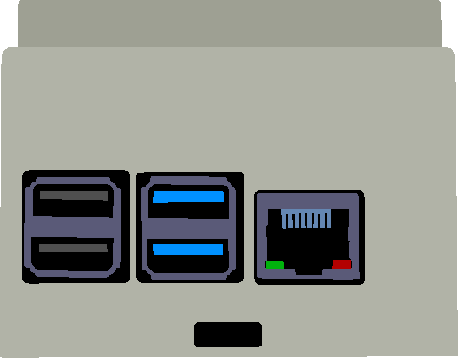
\includegraphics[width=0.6\textwidth]{Title.pdf}
    \vfill
    {\large \lang{Version}{Version}: \GitVersion{} \lang{Stand}{As of}: \PublishDateLocalized{}}\par
\end{titlepage}

\tableofcontents

\vspace{1.5cm}

\lang
{Das \RPI{} sammelt Daten des Solarinvert Wechselrichters. Die Daten können im Browser für verschiedene Zeiträume in unterschiedlichen Darstellungsformen angezeigt werden.}
{The \RPI{} collects data from the Solarinvert inverter. The data can be viewed in a browser for various time periods in different formats.}

\section{\lang{Inbetriebnahme}{Commissioning}}

\lang
{Das \RPI{} existiert in zwei Varianten mit verschiedenen Gehäusen, einmal in einem schwarzen Aluminium Gehäuse (siehe Abbildung~\ref{fig:AluminumHousing}) sowie ein weiteres Modell in einem grauen Gehäuse, das auf einer Hutschiene montiert werden kann (siehe Abbildung~\ref{fig:DinRailHousing}). Die Basis beider Varianten bildet ein Raspberry Pi 4 mit 1 GB RAM.}
{The \RPI{} is available in two versions with different housings: one in a black aluminum housing (see Figure~\ref{fig:AluminumHousing}) and another model in a gray housing that can be mounted on a DIN rail (see Figure~\ref{fig:DinRailHousing}). Both versions are based on a Raspberry Pi 4 with 1 GB of RAM.}

\subsection{\lang{Anschließen}{Connect}}

\begin{figure}[htbp]
    \centering
    \includegraphics[width=126.500mm]{Cable_\Language.pdf}
    \caption{\lang{Kabel}{Cable}}
    \label{fig:Cable}
\end{figure}

\begin{figure}[htbp]
    \centering
    \includegraphics[width=126.500mm]{DinRailHousing_\Language.pdf}
    \caption{\lang{Hutschienengehäuse}{DIN rail enclosure}}
    \label{fig:DinRailHousing}
\end{figure}

\begin{figure}[htbp]
    \centering
    \includegraphics[width=126.500mm]{AluminumHousing_\Language.pdf}
    \caption{\lang{Aluminium Gehäuse}{aluminum enclosure}}
    \label{fig:AluminumHousing}
\end{figure}

\lang
{Das \RPI{} wird mit dem USB-RS485-RJ45 Servicekabel (siehe Abbildung~\ref{fig:Cable} rechts) an den Solarinvert Wechselrichter angeschlossen. Der USB-A Stecker wird dabei in eine USB-Buchse des \RPI{}s (siehe Abbildung~\ref{fig:DinRailHousing} bzw. Abbildung~\ref{fig:AluminumHousing} links) und der RJ45-Stecker in den Wechselrichter gesteckt.}
{The \RPI{} is connected to the solar inverter using the USB-RS485-RJ45 service cable (see Figure~\ref{fig:Cable} on the right). The USB-A plug is inserted into a USB port on the \RPI{} (see Figure~\ref{fig:DinRailHousing} or Figure~\ref{fig:AluminumHousing} on the left), and the RJ45 plug is inserted into the inverter.}

\begin{AttentionBox}
\lang
{Verbinden Sie nicht das \RPI{} und den Wechselrichter mit einem LAN-Kabel über den LAN-Port des \RPI{}s. Nutzen Sie nur das dafür vorgesehene USB-RS485-RJ45 Servicekabel.}
{Do not connect the \RPI{} and the inverter using an LAN cable via the \RPI{}'s LAN port. Use only the USB-RS485-RJ45 service cable provided for this purpose.}
\end{AttentionBox}

\lang
{Versorgen Sie das \RPI{} mit Hilfe des Netzteils (siehe Abbildung~\ref{fig:Cable} links) über den USB-C-Power-Anschluss (siehe Abbildung~\ref{fig:DinRailHousing} bzw. Abbildung~\ref{fig:AluminumHousing} rechts).}
{Power the \RPI{} using the power supply (see Figure~\ref{fig:Cable} on the left) via the USB-C power port (see Figure~\ref{fig:DinRailHousing} or Figure~\ref{fig:AluminumHousing} on the right).}

\subsection{\lang{Herunterfahren}{Shutdown}}

\begin{AttentionBox}
\lang
{Um Schäden am Betriebssystem des \RPI{}s zu vermeiden fahren Sie das System ordnungsgemäß herunter bevor Sie den Strom entfernen.}
{To prevent damage to the \RPI{}'s operating system, shut down the system properly before disconnecting the power.}
\end{AttentionBox}

\lang
{Ziehen Sie dazu den USB-Stecker des USB-RS485-RJ45 Servicekabel aus dem \RPI{} heraus. Nach 100~Sekunden fährt das System herunter. Wenn Sie den USB-Stecker vor Ablauf der 100~Sekunden wieder einstecken, wird der Herunterfahrvorgang nicht durchgeführt.}
{To do this, unplug the USB connector of the USB-RS485-RJ45 service cable from the \RPI{}. The system will shut down after approximately 100~seconds. If you plug the USB connector back in before the 100~seconds have passed, the shutdown process will not be completed.}

\lang
{Man erkennt das Herunterfahren des Systems an dem durchgängigen kurzen Leuchtens der grünen LED. Ist das System Heruntergefahren, ist grüne LED aus und nur die rote LED leuchtet noch. Sie können das \RPI{} nun vom Strom trennen.}{You can tell that the system is shutting down by the steady, brief flashing of the green LED. Once the system has shut down, the green LED is off and only the red LED remains lit. You can now disconnect the \RPI{} from the power source.}

\begin{tabular}{|>{\centering\arraybackslash}p{3.2cm}|
                >{\centering\arraybackslash}p{3cm}|
                >{\centering\arraybackslash}p{3cm}|
                >{\centering\arraybackslash}p{3cm}|}
\hline
& \textbf{\lang{Grüne}{Green} LED} & \textbf{\lang{Rote}{Red} LED} & \textbf{LAN LED} \newline \footnotesize{(\lang{mit LAN verbunden}{connected via LAN})} \\
\hline
\textbf{\lang{Normalbetrieb}{Normal operation}}  & \lang{blinkt langsam}{blinking slowly} &  \lang{durchgehend an}{always on} & \lang{blinkt schnell}{blinking fast} \\
\hline
\textbf{\lang{Herunterfahren}{Shut down now}} & \lang{blinkt schnell}{blinking fast} & \lang{durchgehend an}{always on} & \lang{aus}{off} \\
\hline
\textbf{\lang{Heruntergefahren}{Has shut down}} & \lang{aus}{off}  & \lang{durchgehend an}{always on} & \lang{aus}{off} \\
\hline
\textbf{\lang{Kein Strom}{No power}} & \lang{aus}{off} & \lang{aus}{off} & \lang{aus}{off} \\
\hline
\end{tabular}

\lang
{Um es wieder zu aktivieren, schließen Sie den USB-C-Power-Stecker und den USB-A Stecker des USB-RS485-RJ45 Servicekabel wieder an. Warten Sie mindestens 5~Sekunden zwischen Strom abziehen und wieder anstecken.}
{To reactivate it, reconnect the USB-C power connector and the USB-A connector of the USB-RS485-RJ45 service cable. Wait at least 5~seconds between unplugging and plugging the power back in.}

\lang
{Wird das \RPI{} als reines Windmonitoring ohne Wechselrichter verwendet, dann startet es auch ohne das spezielle USB-RS485 Servicekabel.}
{If the \RPI{} is used solely for wind monitoring without an inverter, it will start up even without the special USB-RS485 service cable.}

\section{\lang{\RPI{} mit dem Heimnetztwerk verbinden}{Connect \RPI{} to the home network}}

\lang
{Das \RPI{} muss mit Ihrem Heimnetzwerk verbunden werden. Dazu können Sie alternativ das \RPI{} mit einem LAN-Kabel zu Ihrem Router verbinden oder das \RPI{} per WLAN mit dem Router verbinden. Es reicht eine von beiden Verbindungsarten.}
{The \RPI{} must be connected to your home network. To do this, you can either connect the \RPI{} to your router using an Ethernet cable or connect the \RPI{} to the router via Wi-Fi. Either connection method is sufficient.}

\subsection{\lang{\RPI{} über LAN Verbinden}{Connecting \RPI{} via LAN}}

\lang
{Verbinden Sie den LAN-Port des \RPI{}s (siehe Abbildung~\ref{fig:DinRailHousing} bzw. Abbildung~\ref{fig:AluminumHousing} links) mit Ihrem Heimnetzwerk per LAN-Kabel.}
{Connect the \RPI{}'s LAN port (see Figure \ref{fig:DinRailHousing} or Figure \ref{fig:AluminumHousing} on the left) to your home network using an Ethernet cable.}

\subsection{\lang{\RPI{} über WLAN Verbinden}{Connect \RPI{} via Wi-Fi}}

\lang
{Sie können den Access Point des \RPI{}s verwenden um dem \RPI{}s die WLAN-Zugangsdaten Ihres Heimnetztwerks bekannt zu machen. Damit der Access Point sichtbar ist darf das \RPI{} nicht per LAN angeschlossen und nicht mit einem WLAN verbunden sein. Sie können ein netzwerkfähiges Gerät (z.B. Handy) nutzen um die Daten einzugeben. Das WLAN des Systems wird zyklisch aktiviert: Es ist jeweils 5~Minuten sichtbar und anschließend 5~Minuten ausgeblendet.}
{You can use the \RPI{}'s access point to configure the \RPI{} to access your home network's Wi-Fi. To make the access point visible, the \RPI{} must not be connected via LAN and must not be connected to another Wi-Fi network. You can use a network-enabled device (e.g., a mobile phone) to enter the settings. The system’s Wi-Fi is activated cyclically: it is visible for 5~minutes and then hidden for 5~minutes.}

\WlanNetwork{\lang{Access Point Zugangsdaten}{Access Point Login Credentials}}{\Logger{}}{\Logger{}!}

\lang
{Öffnen Sie auf Ihrem netzwerkfähigen Gerät die Liste der verfügbaren WLAN-Netzwerke und beobachten Sie die Liste bis zu 5~Minuten, bis das Netzwerk mit der SSID \texttt{\Logger{}} erscheint. Verbinden Sie sich mit dem WLAN-Netzwerk (SSID: \texttt{\Logger{}}) und geben Sie das Passwort \texttt{\Logger{}!} ein.}
{On your network-enabled device, open the list of available Wi-Fi networks and monitor the list for up to 5 minutes until the network with the SSID \texttt{\Logger{}} appears. Connect to the Wi-Fi network (SSID: \texttt{\Logger{}}) and enter the password \texttt{\Logger{}!}.}

\subsubsection{\lang{Connect-Webseite öffnen}{Open the Connect website}}

\lang
{Nachdem Sie mit dem \RPI{} WLAN verbunden sind, öffnet sich bei vielen Geräten automatisch die \textbf{Connect-Webseite} (siehe Abbildung~\ref{fig:ConnectA}).}
{Once you are connected to the \RPI{} Wi-Fi network, the \textbf{Connect website} opens automatically on many devices (see Figure~\ref{fig:ConnectA}).}

\lang
{Falls sich die Webseite nicht automatisch öffnet:}
{If the website does not open automatically:}

\begin{enumerate}
    \item \lang{Öffnen Sie einen Browser (z. B. Chrome, Safari oder Edge).}{Open a web browser (such as Chrome, Safari, or Edge).}
    \item \lang{Geben Sie folgende Adresse ein:}{Enter the following address:} \url{http://192.168.42.1}
\end{enumerate}

\begin{figure}[htbp]
    \centering
    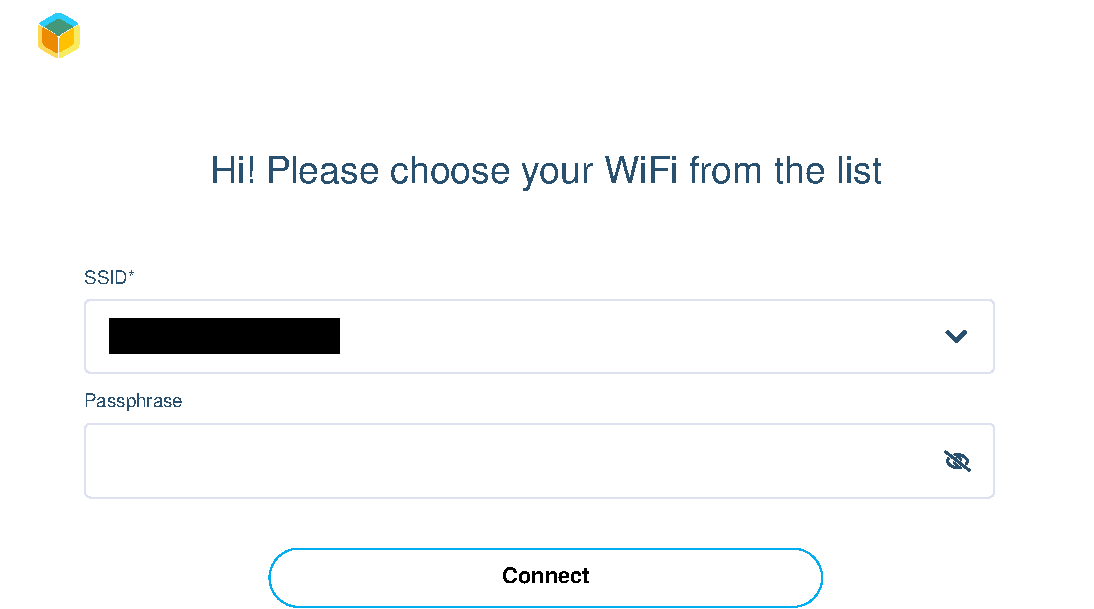
\includegraphics[width=0.6\textwidth]{ConnectA.pdf}
    \caption{\lang{Connect Webseite}{Connect Website}}
    \label{fig:ConnectA}
\end{figure}

\subsubsection{\lang{WLAN-Daten Ihres Netzwerks eingeben}{Connect Website}}

\lang{Tragen Sie die Zugangsdaten Ihres Heim-WLANs ein:}{Enter your home Wi-Fi login credentials:}

\begin{enumerate}
    \item SSID (\lang{Name Ihres WLAN-Netzwerks}{Name of your Wi-Fi network})
    \item \lang{Passwort (WLAN-Passwort Ihres WLAN-Netzwerks)}{Password (the Wi-Fi password for your Wi-Fi network)}
\end{enumerate}

\lang{Diese Informationen finden Sie meist auf der Rückseite Ihres Routers.}{You can usually find this information on the back of your router.}

\lang{Klicken Sie anschließend auf}{Then click} \textbf{Connect}.

\lang{Sie erhalten diese Meldung (siehe Abbildung~\ref{fig:ConnectB}).}{You will see this message (see Figure~\ref{fig:ConnectB}).}

\begin{figure}[htbp]
    \centering
    
\includegraphics[width=0.6\textwidth]{ConnectB.pdf}
    \caption{Connect \lang{Erfolgsmeldung}{Success message}}
    \label{fig:ConnectB}
\end{figure}

\lang
{Das \RPI{} verbindet sich nun mit Ihrem Heim-WLAN. Ihr Gerät kann danach wieder in Ihr normales WLAN wechseln. Falls dies nicht automatisch passiert, verbinden Sie Ihr Gerät einfach wieder mit Ihrem Heim-WLAN.}
{The \RPI{} will now connect to your home Wi-Fi network. Your device can then switch back to your regular Wi-Fi network. If this does not happen automatically, simply reconnect your device to your home Wi-Fi network.}

\subsubsection{\lang{Tipps bei Problemen mit WLAN}{Tips for Troubleshooting Wi-Fi Issues}}

\begin{itemize}
    \item \lang{Das WLAN des \RPI{}s erscheint nicht: Warten Sie bis zu 5~Minuten und aktualisieren Sie die WLAN-Liste.}{The \RPI{}'s Wi-Fi network isn't showing up: Wait up to 5~minutes and refresh the Wi-Fi list.}
    \item \lang{Das WLAN des \RPI{}s erscheint weiterhin nicht: Prüfen Sie, ob der \RPI{} bereits per LAN-Kabel oder mit einem WLAN verbunden ist.}{The \RPI{}'s Wi-Fi network still does not appear: Check whether the \RPI{} is already connected via an Ethernet cable or to a Wi-Fi network.}
    \item \lang{Connect-Webseite öffnet sich nicht: Geben Sie die Adresse \url{http://192.168.42.1} manuell in Ihrem Browser ein.}{The Connect website won't open: Enter the address \url{http://192.168.42.1} manually in your browser.}
\end{itemize}

\section{\lang{Daten anschauen}{View data}}

\lang
{Die Daten können lokal auf dem \RPI{} und auf dem Server angeschaut werden. Dazu können Sie jedes browserfähige Endgerät verwenden.}
{The data can be viewed locally on the \RPI{} and on the server. You can use any device with a web browser to do so.}

\subsection{\lang{Lokal}{Local}}

\lang
{Um die Daten lokal anzuschauen müssen das \RPI{} und Ihr Endgerät zum Betrachten der Daten im selben Heimnetzwerk sein.}
{To view the data locally, the \RPI{} and your device must be on the same home network.}

\lang
{Öffnen Sie den Browser und rufen Sie die Webseite \url{http://\Logger:3000} auf (Wichtig http ohne s und :3000 am Ende).}
{Open your browser and go to the website \url{http://\Logger:3000} (Important: use http without the s and include :3000 at the end).}

\AccessData{\lang{lokal}{local}}{http://\Logger:3000}{admin}{admin}

\subsection{Server}

\lang
{Der Solarinvert Server kann von überall erreicht werden. Öffnen Sie dazu den Browser und rufen Sie die Webseite \url{https://iot.solarinvert.de} auf.}
{The Solarinvert Server can be accessed from anywhere. To do so, open your browser and go to the website \url{https://iot.solarinvert.de}.}

\AccessData{Server}{https://iot.solarinvert.de}{\Logger}{\Password}

\subsection{\lang{Grafana Bedienung}{How to Use Grafana}}

\lang
{Klicken Sie in der linken Leiste auf \textbf{Dashboards}. Ist die linke Leiste nicht da klicken Sie links oben auf das \Icon{GrafanaLogo.pdf}-Symbol um sie einzublenden.}
{Click \textbf{Dashboards} in the left sidebar. If the left sidebar isn't visible, click the \Icon{GrafanaLogo.pdf} icon in the top-left corner to display it.}

\lang
{Unter \textbf{Dashboard} haben Sie in der Mitte mindestens drei Dashboards zur Auswahl.}
{Under \textbf{Dashboard}, you'll find at least three dashboards to choose from in the middle.}


\begin{itemize}
    \item \makebox[2cm][l]{\texttt{Solar:}} \lang{Wenn Sie den Wechselrichter mit Solarpaneelen verwenden.}{If you are using the inverter with solar panels.}
    \item \makebox[2cm][l]{\texttt{Wind:}} \lang{Wenn Sie den Wechselrichter mit einem Windgenerator verwenden.}{If you are using the inverter with a wind turbine.}
    \item \makebox[2cm][l]{\texttt{Wind\_only:}} \lang{Wenn Sie nur Winddaten anschauen möchten.}{If you only want to view wind data.}
\end{itemize}

\lang{Klicken Sie auf das geeignete Dashboard.}{Click on the appropriate dashboard.}

\subsubsection{\lang{Daten regelmäßig aktualisieren}{Update data regularly}}

\lang
{Sie können die Daten der Dashboards regelmäßig aktualisieren in dem Sie links oben neben \textbf{Refresh} auf den Pfeil nach unten klicken (siehe Abbildung~\ref{fig:GrafanaMenu} rechts). Es öffnet sich ein Menü bei dem Sie das gewünschte Zeitintervall auswählen können. Die Daten auf dem Server werden alle 5~Sekunden aktualisiert.}
{You can refresh the dashboard data regularly by clicking the down arrow next to \textbf{Refresh} in the upper-left corner (see Figure~\ref{fig:GrafanaMenu} on the right). A menu will open where you can select the desired time interval. The data on the server is refreshed every 5~seconds.}

\begin{figure}[htbp]
    \centering
    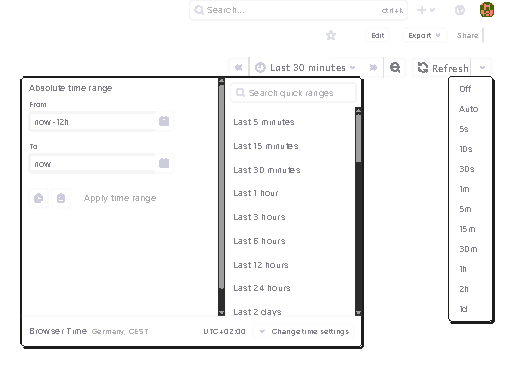
\includegraphics[width=0.6\textwidth]{GrafanaMenu.pdf}
    \caption{Grafana \lang{Menü}{Menu}}
    \label{fig:GrafanaMenu}
\end{figure}

\subsubsection{\lang{Zeit Intervall auswählen}{Select time interval}}

\lang
{Die Daten des Dashboards werden immer für einen bestimmten Zeitbereich angezeigt. Rechts oben (links neben \textbf{Refresh}) wird der aktuelle Zeitbereich angezeigt (siehe Abbildung~\ref{fig:GrafanaMenu} links). Wenn Sie darauf klicken, öffnet sich ein Menü. Sie können dort den gewünschten Zeitbereich auswählen. Wenn Sie auf das \Icon{GrafanaLeft.pdf}-Symbol oder das \Icon{GrafanaRight.pdf}-Symbol klicken können Sie weiter in die Zukunft oder Vergangenheit gehen.}
{The dashboard data is always displayed for a specific time range. The current time range is shown in the top-right corner (to the left of \textbf{Refresh}) (see Figure~\ref{fig:GrafanaMenu} on the left). Clicking on it opens a menu where you can select the desired time range. If you click the \Icon{GrafanaLeft.pdf} icon or the \Icon{GrafanaRight.pdf} icon, you can move further into the future or the past.}

\lang
{Wenn Sie mit gedrückter linker Maustaste in einem Zeitbereich in einem Diagramm einen Bereich markieren, wird dieser Bereich der neue Bereich zum Betrachten.}
{If you select a range in a chart by holding down the left mouse button, that range becomes the new range being displayed.}

\subsubsection{\lang{Dashboard als Vollbild anzeigen}{View the dashboard in full-screen mode}}

\lang
{Klicken Sie rechts oben auf das Runde Icon und wählen Sie dort \textbf{Enable kiosk mode} aus um das Grafana Menü zu verbergen. Drücken Sie \key{F11} um den Browser in Vollbildmodus zu bringen.Drücken Sie \key{ESC} um das Grafana Menü wieder anzuzeigen. Drücken Sie \key{F11} um den Browser wieder in Fenstermodus zu versetzen.}
{Click the round icon in the upper-right corner and select \textbf{Enable kiosk mode} to hide the Grafana menu. Press \key{F11} to enter full-screen mode.Press \key{ESC} to display the Grafana menu again. Press \key{F11} to return the browser to windowed mode.}

\listoffigures

\end{document}
